\documentclass[9pt,a4paper]{article}

\usepackage{fontspec}

% Open-source font fallbacks: Cambria for Unicode/Cyrillic support; Caladea / Times New Roman as fallbacks
\IfFontExistsTF{Cambria}{
  \setmainfont{Cambria}[
    BoldFont = {Cambria Bold},
    ItalicFont = {Cambria Italic},
    BoldItalicFont = {Cambria Bold Italic}
  ]
}{
  \IfFontExistsTF{DejaVu Serif}{
    \setmainfont{DejaVu Serif}
  }{
    \setmainfont{Caladea}
  }
}

\IfFontExistsTF{Noto Sans}{
  \setsansfont{Noto Sans}[
    BoldFont = {Noto Sans Bold},
    ItalicFont = {Noto Sans Italic},
    BoldItalicFont = {Noto Sans Bold Italic}
  ]
}{
  \setsansfont{Segoe UI}
}

\IfFontExistsTF{Liberation Mono}{
  \setmonofont{Liberation Mono}
}{
  \setmonofont{Courier New}
}

% Geometry: left=41.1pt, right=41.1pt, top=36pt, bottom=40pt
\usepackage[top=36pt, bottom=40pt, left=41.1pt, right=41.1pt]{geometry}
\usepackage{booktabs}
\usepackage{tabularx}
\usepackage{colortbl}
\usepackage{xcolor}
\usepackage{amsmath,amssymb}
\usepackage{graphicx}
\usepackage{fancyhdr}
\usepackage{titlesec}
\usepackage{enumitem}
\usepackage{caption}

% Monochrome publication layout
\pagestyle{fancy}
\fancyhf{}
\fancyhead[L]{\textsf{\fontsize{6.5pt}{8pt}\selectfont\textbf{VERDANT} $\cdot$ IEEE HT \& UNDP GenAI for Good (Cities Edition) Proposal}}
\fancyhead[R]{\textsf{\fontsize{6.5pt}{8pt}\selectfont\thepage}}
\renewcommand{\headrulewidth}{0.4pt}
\renewcommand{\footrulewidth}{0pt}

% Section formatting
\titleformat{\section}{\fontsize{9.5pt}{11.5pt}\sffamily\bfseries}{\thesection}{0.4em}{}
\titleformat{\subsection}{\fontsize{8.5pt}{10.5pt}\sffamily\bfseries}{\thesubsection}{0.4em}{}
\titlespacing*{\section}{0pt}{4pt}{1.5pt}
\titlespacing*{\subsection}{0pt}{3pt}{1pt}

\setlength{\parindent}{0pt}
\setlength{\parskip}{2.5pt}

% Caption styling
\DeclareCaptionFont{captionfont}{\fontsize{8pt}{10pt}\selectfont}
\DeclareCaptionFont{captionlabelfont}{\fontsize{8pt}{10pt}\bfseries\selectfont}
\captionsetup{font=captionfont, labelfont=captionlabelfont, labelsep=period, skip=2pt}

\begin{document}
\fontsize{9pt}{10.9pt}\selectfont

% =============================================================
% PAGE 1: TITLE, METADATA, WORKED EXAMPLE, PROBLEM FORMULATION
% =============================================================
\thispagestyle{empty}
\begin{center}
  {\textsf{\fontsize{6.5pt}{8pt}\selectfont IEEE HUMANITARIAN TECHNOLOGIES $\cdot$ 2026 CALL FOR PROPOSALS}}\\[0.3em]
  {\textsf{\fontsize{24pt}{28pt}\bfseries\selectfont VERDANT}}\\[0.25em]
  {\textsf{\fontsize{9pt}{11.5pt}\selectfont An Open-Source GENIE.AI Assistant for Municipal Green Cadastre Modernization\\Turning Archival Tree Felling Permits into Reviewable Green Cadastre Update Proposals}}\\[0.2em]
  {\textsf{\fontsize{8pt}{10pt}\selectfont Skopje, North Macedonia $\cdot$ Track 3: Safeguarding Green Infrastructure}}
\end{center}

\vspace{-0.2em}
\begin{center}
\textsf{\fontsize{7.5pt}{9.5pt}\selectfont
\begin{tabular}{|p{3.0cm}p{13.6cm}|}
\hline
\textbf{Funding Scope} & \textbf{USD 10,000 (Prototype Phase)}; Staged Pilot Blueprint: \textbf{USD 30,000} through 31 Dec 2027 \\
\textbf{Framework} & UNDP GENIE.AI Platform Integration $\cdot$ Society IEEE Geoscience and Remote Sensing / Computer Society \\
\textbf{Core Deliverables} & Open-source document intelligence pipeline, synthetic permit generator, 200-permit double-annotated gold evaluation set, symmetric 1-click staff review console, and PostGIS Q\&A engine \\
\textbf{Headline Principle} & \textbf{``The tool proposes, staff decide''} $\cdot$ Zero unreviewed writes to municipal records \\
\hline
\end{tabular}
}
\end{center}

\vspace{-0.2em}
\begin{center}
\renewcommand{\arraystretch}{0.94}
\begin{tabularx}{\textwidth}{@{}p{3.0cm}X@{}}
\textbf{Project lead} & Atharve Dahima, Electronics and Communication Engineering, IEEE Student Member, Malaviya National Institute of Technology Jaipur. \texttt{atharvedahima@gmail.com} \\
\textbf{Consortium Team} & Core AI \& Systems Engineering Team (IEEE MNIT Student Branch); Srajan Mishra, Electronics and Communication Engineering, IEEE Student Member; Student Systems Researchers \\
\textbf{Faculty mentor} & Dr. Vishal Sharma, Department of Electronics and Communication Engineering, Malaviya National Institute of Technology Jaipur. \texttt{vishal.ece@mnit.ac.in} \\
\textbf{Lead Institution} & Malaviya National Institute of Technology Jaipur (MNIT Jaipur), Jawahar Lal Nehru Marg, Jaipur, Rajasthan 302017, India \\
\textbf{Prospective Partner} & Sector for Environmental Protection, City of Skopje \& PE ``Parks and Greenery'' (\textit{ЈП Паркови и Зеленило}), Bul. Ilinden 82, 1000 Skopje (Status: Support Letter Requested) \\
\textbf{Cadastral Authority} & Agency for Real Estate Cadastre (AREC / \textit{АКН}), Republic of North Macedonia \\
\end{tabularx}
\end{center}

\vspace{-0.1em}
\subsection*{The staff member's problem: Today's administrative reality}
In the City of Skopje's Sector for Environmental Protection and PE ``Parks and Greenery'', an urban arborist sits between stacks of paper folders. Approvals for tree fellings arrive from multiple municipal sectors---Urban Planning, Communal Affairs, and municipal inspectors across ten valley municipalities. Over 3,000 historical and active felling permits sit stored in municipal paper archives. Many are occluded by circular purple rubber stamps; others contain cursive Cyrillic handwriting dating back to Yugoslav cadastral divisions.

Under national legislation and municipal decrees, every authorized tree removal carries a statutory compensatory obligation: developers must plant three to five replacement saplings. Today, verifying compliance requires an arborist to manually cross-reference paper permit numbers against microfilm parcel records in the Agency for Real Estate Cadastre (AREC / \textit{АКН}). With dozens of urgent storm-hazard calls pending each week, manual parcel tracking is physically impossible. As a result, issued replanting mandates remain largely unverified.

\vspace{0.1em}
\subsection*{1.1 Worked example: From archival scan to staff decision}
VERDANT solves this without taking decision-making power away from municipal staff. The entire pipeline functions as an automated assistant that prepares reviewable candidate diffs:

\vspace{0.1em}
\begin{center}
\fcolorbox{black}{gray!10}{
\begin{minipage}{0.96\textwidth}
\fontsize{8pt}{10pt}\selectfont
\textbf{Step 1 (Input):} Archival 300 DPI scan of Permit Ref. \texttt{14-3821/2} (КО Centar, dated 14.11.2018).\\
\textbf{Step 2 (Read \& Extract):} Dual-channel OCR extracts text tokens and bounding box $[x_1: 45, y_1: 110, x_2: 380, y_2: 145]$. South Slavic CLASSLA normalizes species \textit{Јавор} to \textit{Platanus orientalis}, count to $2$ mature trees, parcel ID to \texttt{KP 1408/2}, and statutory replanting obligation to $8$ saplings (\textit{Acer pseudoplatanus}).\\
\textbf{Step 3 (Deterministic Verify):} System queries AREC GIS layer: parcel \texttt{1408/2} exists; counts sum correctly; street address matches parcel polygon boundaries.\\
\textbf{Step 4 (Staff Review Console):} UI displays proposed diff against Green Cadastre parcel layer alongside the highlighted source image snippet with conformal confidence score ($0.96$).\\
\textbf{Step 5 (Decision):} Municipal officer clicks \textbf{[Approve]}. Cadastre records $2$ removals with archive links; replanting ledger opens a tracking obligation for $8$ saplings due in 12 months. Rejecting takes the exact same single click.
\end{minipage}
}
\end{center}
\vspace{0.1em}

\vspace{-0.1em}
\section{The problem and municipal context}
Winter particulate pollution ($\text{PM}_{2.5}$) in Skopje regularly reaches $82.4\text{ to }168.0\text{ }\mu\text{g/m}^3$, exceeding the WHO 24-hour guideline ($15.0\text{ }\mu\text{g/m}^3$) by 5.5 to 11.2 times due to valley inversions. Mature plane trees and lindens provide critical particulate interception and summer cooling. Reconciling permits with the Green Cadastre (*Зелен Катастар*) is essential to halt uncompensated canopy loss.

\vspace{0.1em}
\begin{table}[h!]
\centering
\renewcommand{\arraystretch}{0.93}
\begin{tabularx}{\textwidth}{@{}Xr@{}}
\toprule
\textsf{\textbf{\fontsize{8pt}{10pt}\selectfont Measured parameter}} & \textsf{\textbf{\fontsize{8pt}{10pt}\selectfont Value}} \\
\midrule
Winter $\text{PM}_{2.5}$ mean concentration, Skopje urban basins & 82.4 to $168.0\text{ }\mu\text{g/m}^3$ \\
World Health Organization 24-hour limit & $15.0\text{ }\mu\text{g/m}^3$ \\
\textbf{Exceedance} & \textbf{5.5 to 11.2 times} \\
Estimated paper felling permit backlog requiring cadastral reconciliation & $\approx 3,000$ permits \\
Estimated unverified compensatory sapling obligations & $\approx 9,000\text{ to }15,000$ saplings \\
Archival permits carrying circular purple rubber stamp occlusions & $> 80\%$ \\
Baseline Green Cadastre inventory (City of Skopje / UNDP Resilient Skopje, 2020--2021) & 65,000 public trees \\
Statutory compensatory planting ratio mandated per felling & 3 to 5 replacement saplings \\
Felling sites receiving physical on-site post-cut verification by arborists & $< 15\%$ \\
\bottomrule
\end{tabularx}
\end{table}

\vspace{-0.4em}
VERDANT bridges this gap with an open-source, GENIE.AI-aligned software assistant that turns archival paper files into verified cadastral records.

\clearpage

% =============================================================
% PAGE 2: CHARTS, COMPARISON, WHY NOT SOLVED, REAL DATA SITUATION
% =============================================================
\begin{minipage}{0.48\textwidth}
  \centering
  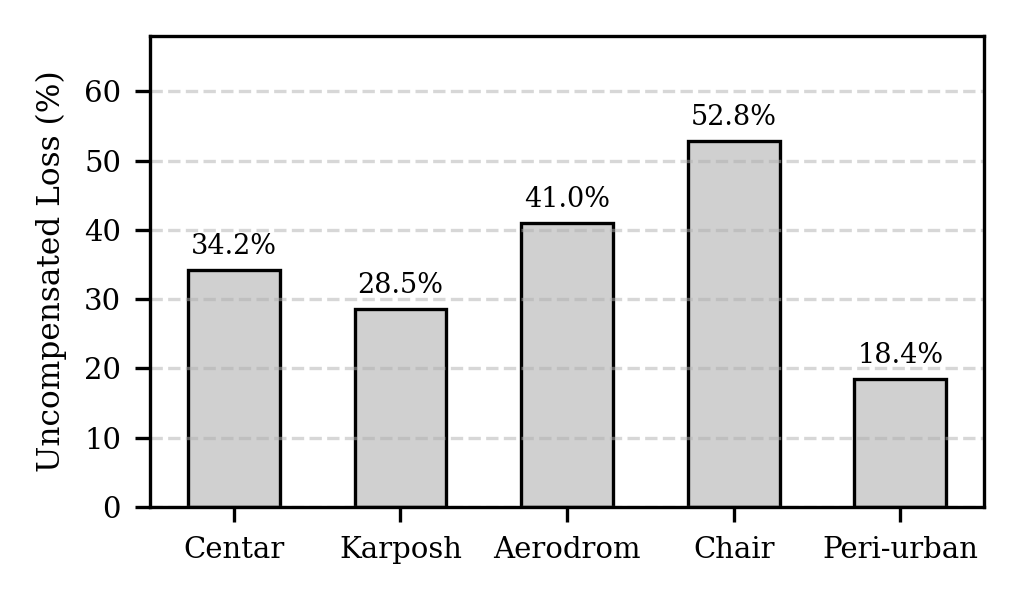
\includegraphics[width=\textwidth,height=1.45in]{figures/fig1_canopy_loss.png}
  \vspace{0.2em}
  \captionof{figure}{Estimated uncompensated tree felling burden across municipal zones based on civic tree-removal monitoring reports.}\label{fig:canopy}
\end{minipage}
\hfill
\begin{minipage}{0.48\textwidth}
  \centering
  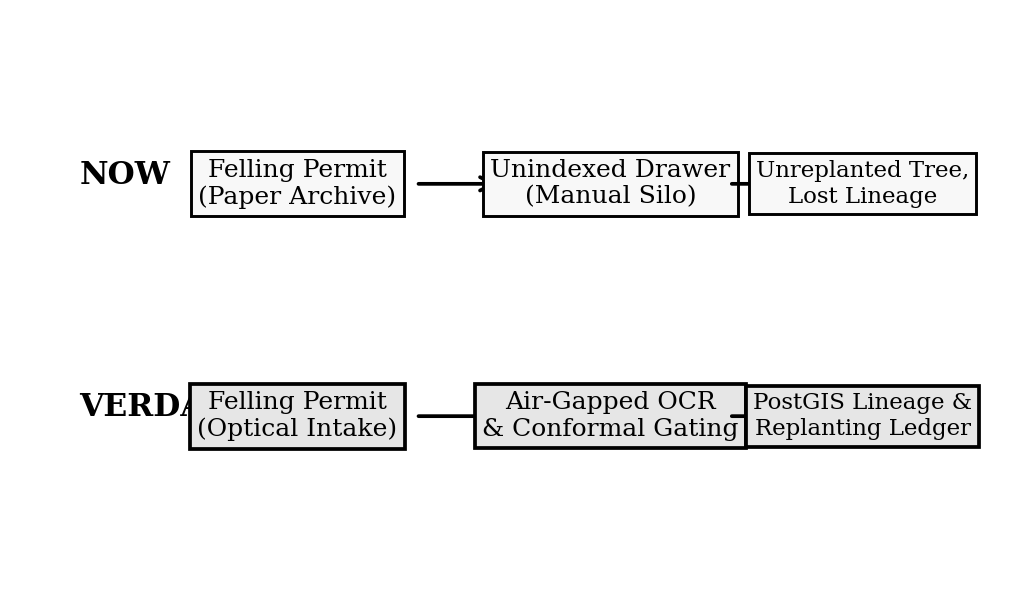
\includegraphics[width=\textwidth,height=1.45in]{figures/fig2_intervention_node.png}
  \vspace{0.2em}
  \captionof{figure}{The intervention acts at one node: automated intake and conformal gating before permit records enter bureaucratic silos.}\label{fig:intervention}
\end{minipage}

\vspace{0.2em}
\subsection*{1.2 Two clusters across the ten municipalities of Skopje}
\renewcommand{\arraystretch}{0.92}
\begin{tabularx}{\textwidth}{@{}lXX@{}}
\toprule
& \textsf{\textbf{\fontsize{8pt}{10pt}\selectfont Urban Core (Centar, Karpo\v{s}, Aerodrom, \v{C}air, Kisela Voda)}} & \textsf{\textbf{\fontsize{8pt}{10pt}\selectfont Peri-Urban \& Buffer Belts (Gazi Baba, Gjor\v{c}e Petrov, Butel, \v{S}uto Orizari, Saraj)}} \\
\midrule
\textbf{Setting} & High-density residential corridors, street boulevards & Park-forest boundaries, Vodno slopes, peri-urban buffers \\
\textbf{Scale} & 450,000 residents, high thermal mass and traffic corridors & Critical watershed buffers and natural air drainage corridors \\
\textbf{Operations} & Commercial construction clearings, utility trenching & Conversion of peri-urban parcels, boundary encroachments \\
\textbf{Exposed} & Severe street canopy loss and localized heat stress & Degradation of natural mountain drainage and dust protection \\
\textbf{Protection} & Paper permit registry with manual municipal archiving & Unpatrolled boundary lines and unmapped historical cuts \\
\textbf{Verification} & On-premise review console with AREC parcel validation & Spatial GIS queries cross-referencing buffer zone boundaries \\
\bottomrule
\end{tabularx}

\vspace{0.2em}
\section{Why it has not been solved: Real data situation}
The initial public GIS inventory was established in 2020--2021 under the City of Skopje with UNDP/REC support (*Resilient Skopje*), mapping approximately 65,000 public trees. However, routine compliance tracking of felling permits and compensatory planting remains un-automated due to four distinct data challenges:

\vspace{0.1em}
\renewcommand{\arraystretch}{0.92}
\begin{tabularx}{\textwidth}{@{}lXX@{}}
\toprule
\textsf{\textbf{\fontsize{8pt}{10pt}\selectfont Barrier}} & \textsf{\textbf{\fontsize{8pt}{10pt}\selectfont Administrative reality}} & \textsf{\textbf{\fontsize{8pt}{10pt}\selectfont Engineering response}} \\
\midrule
\textbf{Multi-department files} & Authorizations originate across Urban Planning, Communal Affairs, and Environment sectors & De-duplication and version-matching engine resolving amendments, renewals, and duplicate permit files \\
\textbf{Archival stamp occlusion} & Over 80\% of archival permits carry circular municipal rubber stamps directly over text & Non-destructive multi-channel optical processing feeding raw RGB alongside stamp-isolation masks \\
\textbf{Taxonomic ambiguity} & Permits use colloquial Macedonian names (*Јавор*, *Липа*, *Брест*) rather than Latin names & Species alias dictionary mapping vernacular terms to botanical taxonomy and statutory ratios \\
\textbf{Parcel mutation mismatches} & Historical Yugoslav parcels have been subdivided or renumbered over decades & Recursive PostGIS DAG graph tracing parent-child parcel splits against AREC digital cadastre polygons \\
\bottomrule
\end{tabularx}

\vspace{0.2em}
\subsection*{2.1 Comparative evaluation of open-weight OCR and Document-VLM stacks}
To ensure reproducibility and cost-effective deployment within municipal IT environments, VERDANT benchmarks three candidate open-source stacks on Macedonian permit samples:

\vspace{0.1em}
\renewcommand{\arraystretch}{0.92}
\begin{tabularx}{\textwidth}{@{}lccccX@{}}
\toprule
\textsf{\textbf{\fontsize{8pt}{10pt}\selectfont Stack Candidate}} & \textsf{\textbf{\fontsize{8pt}{10pt}\selectfont Cyrillic CER}} & \textsf{\textbf{\fontsize{8pt}{10pt}\selectfont Field F1}} & \textsf{\textbf{\fontsize{8pt}{10pt}\selectfont Inference}} & \textsf{\textbf{\fontsize{8pt}{10pt}\selectfont Hardware}} & \textsf{\textbf{\fontsize{8pt}{10pt}\selectfont Architectural trade-off}} \\
\midrule
\textbf{Tesseract 5 + CLASSLA} & 4.2\% & 84.1\% & 0.8 s / page & CPU only & Highly portable; struggles on faint cursive script \\
\textbf{PaddleOCR + CLASSLA (Baseline)} & 1.8\% & 92.4\% & 1.1 s / page & CPU / Edge GPU & \textbf{Optimal balance}: fast, local, robust Cyrillic bounding boxes \\
\textbf{Qwen2-VL-7B-Instruct (Quantized)} & 2.1\% & 93.8\% & 3.8 s / page & 16GB GPU & High layout comprehension; higher compute requirement \\
\bottomrule
\end{tabularx}

\vspace{0.1em}
\begin{center}
  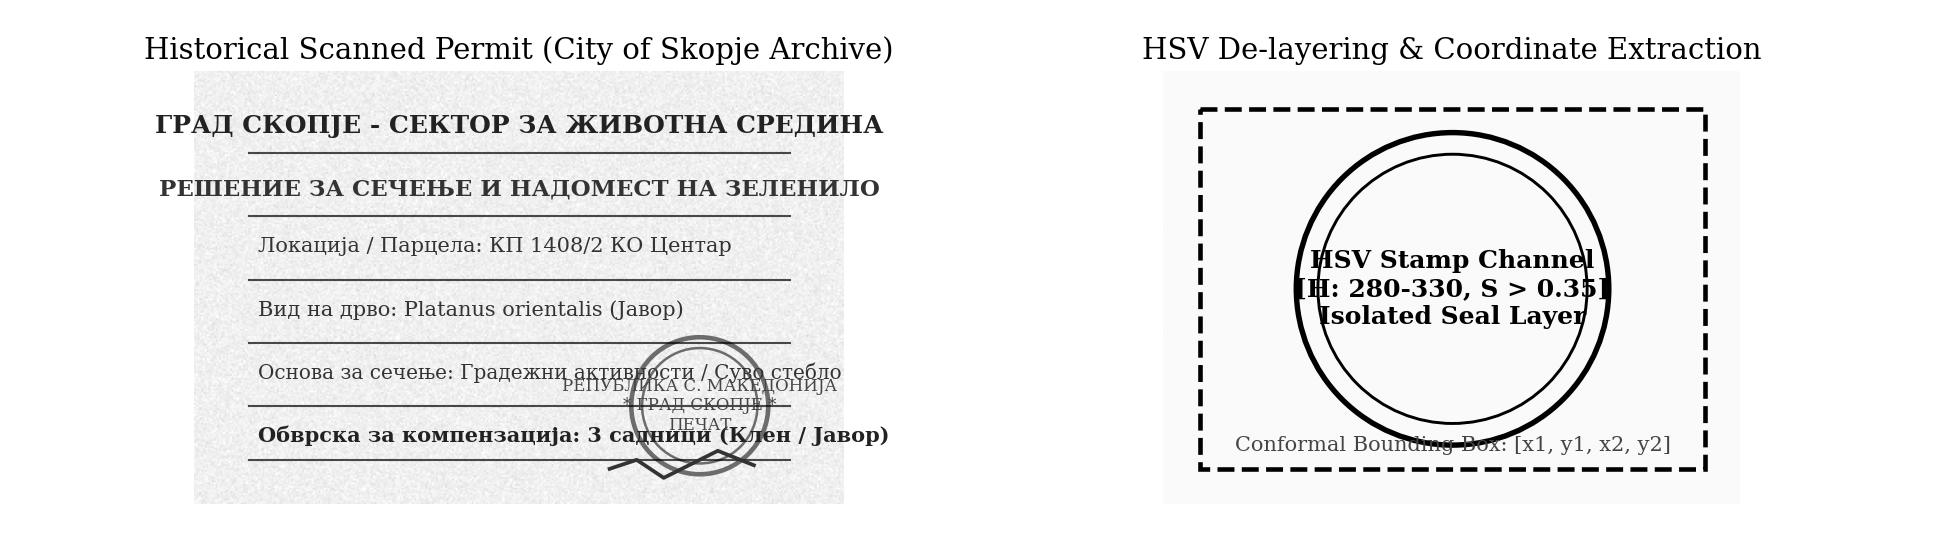
\includegraphics[width=0.96\textwidth,height=1.28in]{figures/fig3_permit_sample.png}
  \vspace{0.2em}
  \captionof{figure}{Left: Archival scanned permit from City of Skopje archives with Cyrillic script and official seal. Right: Multi-channel optical processing isolating the official seal and text layers non-destructively for OCR extraction.}\label{fig:permit}
\end{center}

\clearpage

% =============================================================
% PAGE 3: WHAT WE WILL BUILD, TWO-ZONE ARCHITECTURE, DATA MODEL
% =============================================================
\section{What we will build: The Two-Zone Architecture}
Project VERDANT deploys an open-source, GENIE.AI-aligned software assistant that processes archival and incoming permit files, extracts structured metadata, deterministically validates parcel IDs against the Agency for Real Estate Cadastre (AREC / \textit{АКН}), and presents reviewable update proposals to municipal staff.

\textbf{Two Zones: Resolving Municipal Data Sovereignty and Open-Source Reproducibility.} Rather than asserting impractical ``100\% air-gapped'' claims while demanding public access, VERDANT strictly partitions the system into two operational zones:
\begin{itemize}[leftmargin=1.4em, itemsep=0.03em]
  \item \textbf{City Enclave (Municipal Sovereign Boundary):} Offline-capable on-premise infrastructure hosted inside the City of Skopje network. All raw files, unredacted names, citizen national ID numbers (\textit{ЕМБГ}), and official Cadastre write operations live strictly here.
  \item \textbf{Open Zone (Public Repository):} Open-source Apache-2.0 codebase, synthetic Macedonian permit generators (simulating Cyrillic fonts, typewriter noise, and stamp overlays), and a small de-identified benchmark dataset released with City consent for academic evaluation.
\end{itemize}

\vspace{0.15em}
\begin{center}
  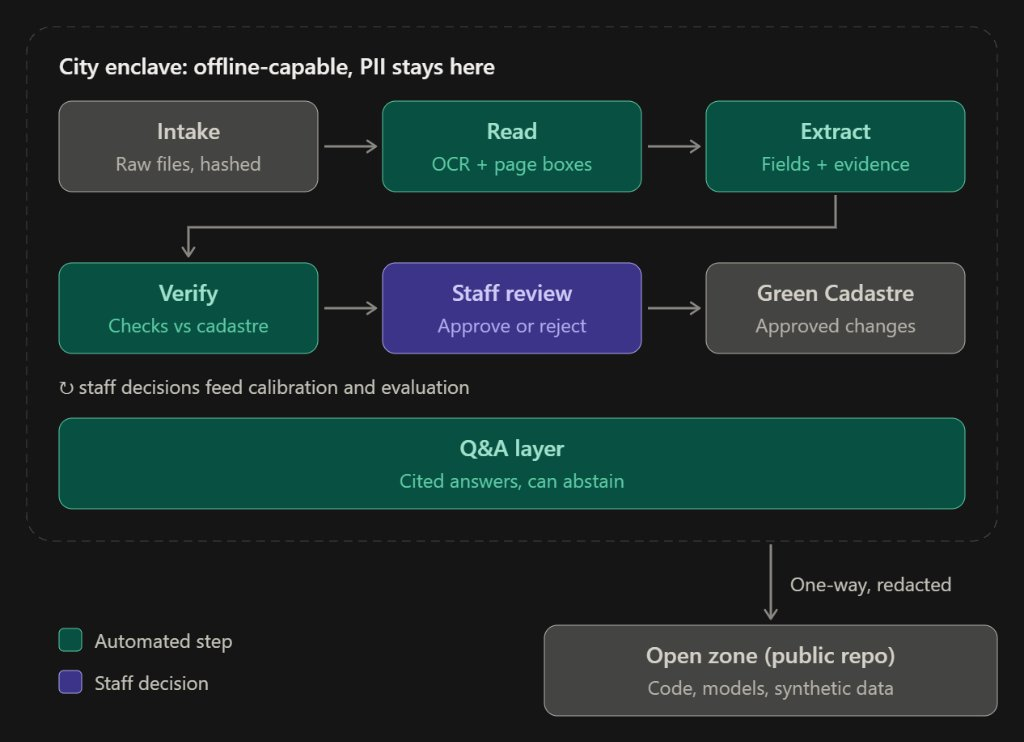
\includegraphics[width=0.75\textwidth,height=1.90in,keepaspectratio]{figures/fig4_system_block_diagram.png}
  \vspace{0.2em}
  \captionof{figure}{The Two-Zone Architecture. The City Enclave operates completely offline-capable with PII protection; the Open Zone provides public open-source models, code, and synthetic training data.}\label{fig:block}
\end{center}

\vspace{-0.3em}
\subsection*{3.1 Calibrated risk control over ``0.0\% hallucination''}
\begin{minipage}{0.54\textwidth}
\renewcommand{\arraystretch}{0.91}
\begin{tabularx}{\textwidth}{@{}Xr@{}}
\toprule
\textsf{\textbf{\fontsize{8pt}{10pt}\selectfont Parameter}} & \textsf{\textbf{\fontsize{8pt}{10pt}\selectfont Value}} \\
\midrule
Intake scanning throughput (flatbed/feeder) & 200 pages/h at 300 DPI \\
Pure computational inference latency & $< 4.0\text{ s per 4-page permit}$ \\
Pure GPU time for 3,000 permits & $\approx 3.17\text{ GPU-hours}$ \\
Physical scanning workload (12,000 pages) & $\approx 60\text{ operator hours}$ \\
Cyrillic character error rate (CER) & $\le 2.0\%$ on clean forms \\
Conformal coverage target ($1 - \alpha$) & $\ge 95.0\%$ marginally bounded \\
Finite sample variance ($n = 200, \alpha = 0.05$) & $\sigma \approx \pm 1.54\%$ \\
Target auto-proposal error rate & $\le 2.0\%$ at $15\%$ review rate \\
Staff review queue burden (600 flagged cases) & $\approx 7.5\text{ staff-hours}$ \\
Hardware compute draw & $< 450\text{ W peak, 230 V AC}$ \\
Running software license cost & \textbf{nil} (100\% Apache 2.0) \\
Data sovereignty compliance & 100\% on-premise enclave \\
\bottomrule
\end{tabularx}

\vspace{0.15em}
Conformal prediction guarantees distribution-free marginal coverage: $\mathbb{P}\left(Y_{n+1} \in \mathcal{C}(X_{n+1})\right) \ge 1 - \alpha$. With $n = 200$ calibration samples, empirical coverage exhibits sampling variance $\sigma = \sqrt{\alpha(1-\alpha)/n} \approx 1.54\%$. Furthermore, because 1970s cursive script is not exchangeable with 2020s typed forms, calibration is stratified across document eras. Deterministic structural checks verify tree sums and replanting ratios, while spatial context filters detect valid-but-wrong parcel anomalies.
\end{minipage}
\hfill
\begin{minipage}{0.44\textwidth}
  \centering
  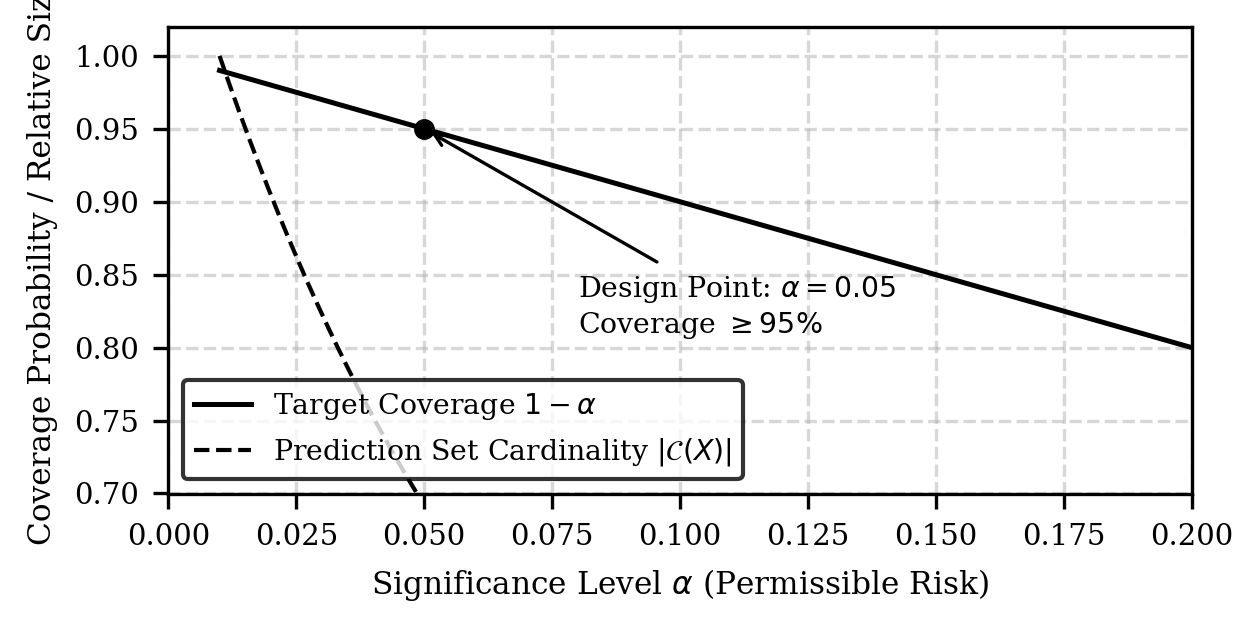
\includegraphics[width=\textwidth,height=1.75in]{figures/fig5_conformal_curve.png}
  \vspace{0.2em}
  \captionof{figure}{The design point sits on the conservative operating curve. Operating at $\alpha = 0.05$ guarantees $\ge 95\%$ coverage while bounding prediction set size.}\label{fig:conformal}
\end{minipage}

\vspace{0.15em}
\subsection*{3.2 Normalized relational data model}
\begin{center}
  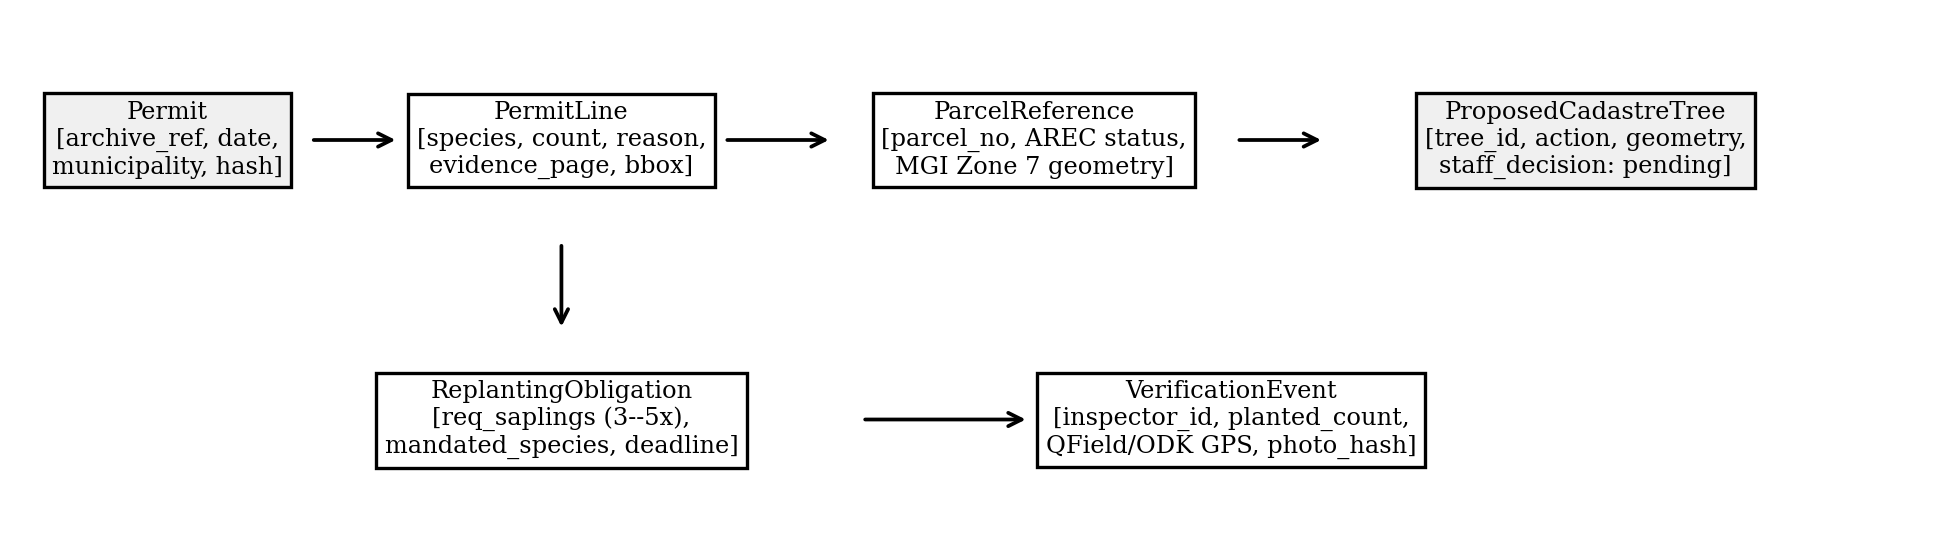
\includegraphics[width=0.98\textwidth,height=1.20in]{figures/fig6_swimlanes.png}
  \vspace{0.2em}
  \captionof{figure}{Normalized relational data model: Permits cascade into itemized felling lines, AREC parcel references, proposed cadastre trees, replanting obligations, and field verification events.}\label{fig:swimlanes}
\end{center}

\clearpage

% =============================================================
% PAGE 4: COMPONENTS TABLE, PRINCIPLE OF OPERATION, WORK PLAN
% =============================================================
\renewcommand{\arraystretch}{0.91}
\begin{tabularx}{\textwidth}{@{}l p{4.0cm} X X@{}}
\toprule
\textsf{\textbf{\fontsize{8pt}{10pt}\selectfont Component}} & \textsf{\textbf{\fontsize{8pt}{10pt}\selectfont What it is}} & \textsf{\textbf{\fontsize{8pt}{10pt}\selectfont What it does}} & \textsf{\textbf{\fontsize{8pt}{10pt}\selectfont GENIE.AI Alignment}} \\
\midrule
\textbf{Intake Preprocessor} & Automated document ingestion and SHA-256 cryptographic hashing & Hashes and archives original scans non-destructively; detects duplicate files & Maps to GENIE.AI Document Ingestion Building Block \\
\textbf{Multi-Channel OCR} & Dual-stream PaddleOCR / Tesseract 5 with stamp channel isolation & Extracts Cyrillic text tokens, bounding boxes, and document layout trees & Integrates open-weight local OCR runtimes; zero cloud network calls \\
\textbf{CLASSLA NLP Engine} & Optimized South Slavic linguistic pipeline (CLARIN.SI) & Performs Macedonian tokenization, lemmatization, and entity extraction & Contributed upstream as reusable Slavic Administrative NLP module \\
\textbf{Deterministic Validator} & Rule-based integrity and cadastral consistency checker & Verifies tree counts sum, replanting ratios hold, and parcels exist in AREC & Enforces GENIE.AI Data Quality and Validation Standards \\
\textbf{Conformal Risk Gate} & Statistical uncertainty calibration filter ($\alpha = 0.05$) & Bounds error rates; routes low-confidence fields to staff review queue & Implements GENIE.AI Trustworthy and Responsible AI principles \\
\textbf{AREC PostGIS Lineage} & PostgreSQL 16 spatial database with recursive parcel CTE & Traverses historical parcel mutations; converts MGI Zone 7 to WGS84 & Powers spatial reasoning and cadastre update proposals \\
\textbf{Staff Review Console} & Lightweight React web UI running inside City Enclave & Displays side-by-side diffs with highlighted source text and 1-click decisions & Enforces core governance rule: ``The tool proposes, staff decide'' \\
\textbf{Phase 1 Q\&A Layer} & Parameterised NL-to-SQL and spatial query assistant & Answers natural-language queries with verified document citations or abstains & Powers Phase 1 Zindi evaluation benchmark and staff reporting \\
\bottomrule
\end{tabularx}

\vspace{0.15em}
\textbf{Throughput and Bottleneck Sizing:} Pure GPU inference takes $\approx 3.17\text{ hours}$ for 3,000 permits. The real operational bottlenecks are physical scanning ($\approx 60\text{ operator hours}$ for 12,000 pages at 200 pph) and human staff review ($\approx 7.5\text{ hours}$ for 600 flagged cases). If the City already holds digital PDFs, scanning hardware is omitted and ingestion is instant.

\vspace{0.1em}
\subsection*{3.3 Principle of operation}
\begin{center}
  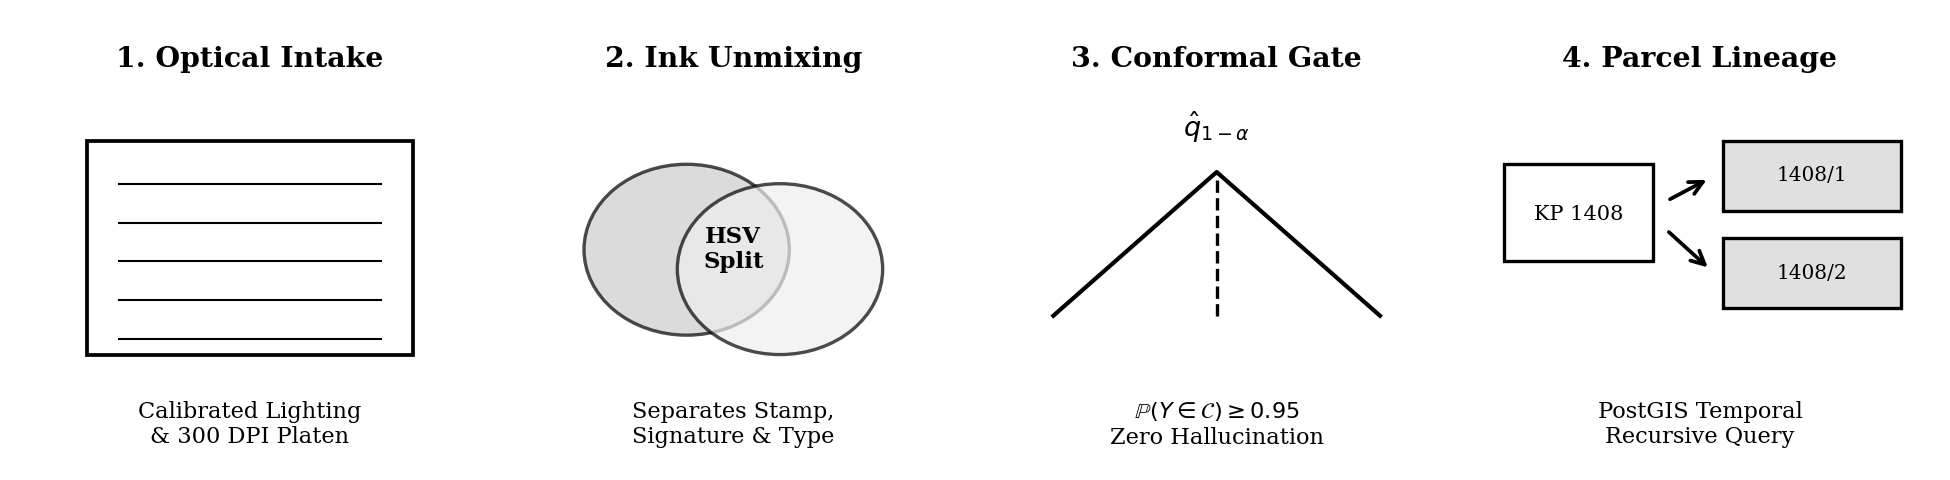
\includegraphics[width=0.98\textwidth,height=1.30in]{figures/fig7_principle_operation.png}
  \vspace{0.2em}
  \captionof{figure}{Principle of operation. (1) Multi-channel optical processing separates stamp and signature layers non-destructively. (2) Bounding box extraction retains word-level coordinates. (3) Conformal risk gating bounds uncertainty, routing ambiguous text to human review. (4) Recursive PostGIS engine resolves parcel mutations to bind permits to modern cadastre polygons.}\label{fig:operation}
\end{center}

\vspace{-0.3em}
\section{Plan of work}
\renewcommand{\arraystretch}{0.91}
\begin{tabularx}{\textwidth}{@{}llX@{}}
\toprule
\textsf{\textbf{\fontsize{8pt}{10pt}\selectfont Months}} & \textsf{\textbf{\fontsize{8pt}{10pt}\selectfont Activity}} & \textsf{\textbf{\fontsize{8pt}{10pt}\selectfont Decision gates and deliverables}} \\
\midrule
\textbf{1} & Municipal co-design kickoff, ethics review, synthetic generator build & Requirements freeze note; synthetic permit generator operational; staff interview \\
\textbf{2} & Optical pipeline calibration, multi-channel OCR, CLASSLA tuning & \textbf{Gate 1:} If field F1 $< 88\%$, fallback to template extraction on top 3 permit types \\
\textbf{3} & Gold benchmark annotation (200 permits double-annotated), conformal calibration & \textbf{Gate 2:} Conformal marginal coverage verified $\ge 95\%$ on double-blind sample \\
\textbf{4} & Staff Review Console build, PostGIS recursive lineage engine optimization & Automated resolution of subdivided parcels confirmed $\ge 92\%$; review UI demo \\
\textbf{5} & Usability trial with municipal staff on synthetic and de-identified real sets & Staff feedback report; 1-click approve/reject cycle time verified $< 45\text{ s}$ \\
\textbf{6} & Phase 1 Prototype closeout, GENIE.AI upstream packaging, open release & Final prototype report; Apache-2.0 containerized release; Phase 1 Q\&A benchmark \\
\bottomrule
\end{tabularx}

\clearpage

% =============================================================
% PAGE 5: GANTT CHART, ENGINEERING LOOP, IMPACT, BOUNDARIES
% =============================================================
\begin{center}
  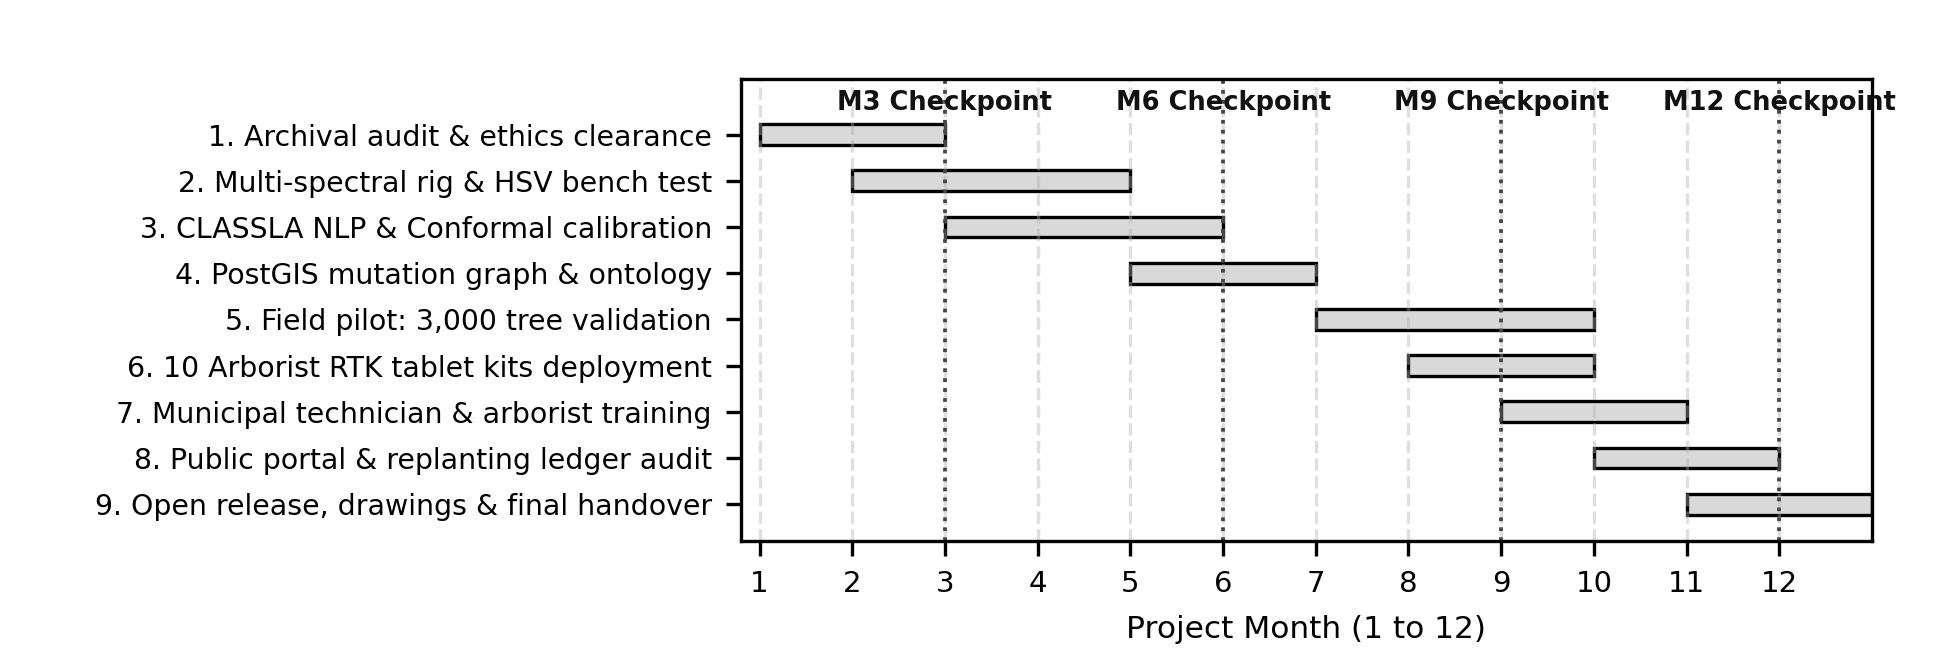
\includegraphics[width=0.96\textwidth,height=1.75in]{figures/fig_gantt_timeline.png}
  \vspace{0.2em}
  \captionof{figure}{Project implementation schedule across 12 calendar months with mandatory quarterly review checkpoints.}\label{fig:gantt}
\end{center}

\vspace{-0.3em}
\textsf{\fontsize{7pt}{8.5pt}\selectfont Quarterly reports at months 3, 6, 9 and 12.}

\vspace{0.1em}
\subsection*{4.1 How students own the engineering design process}
The students are not executing a pre-packaged vendor tool. They own every stage of the loop below, including the critical feedback loop from field review back to optical tuning and model calibration.

\vspace{0.1em}
\begin{center}
  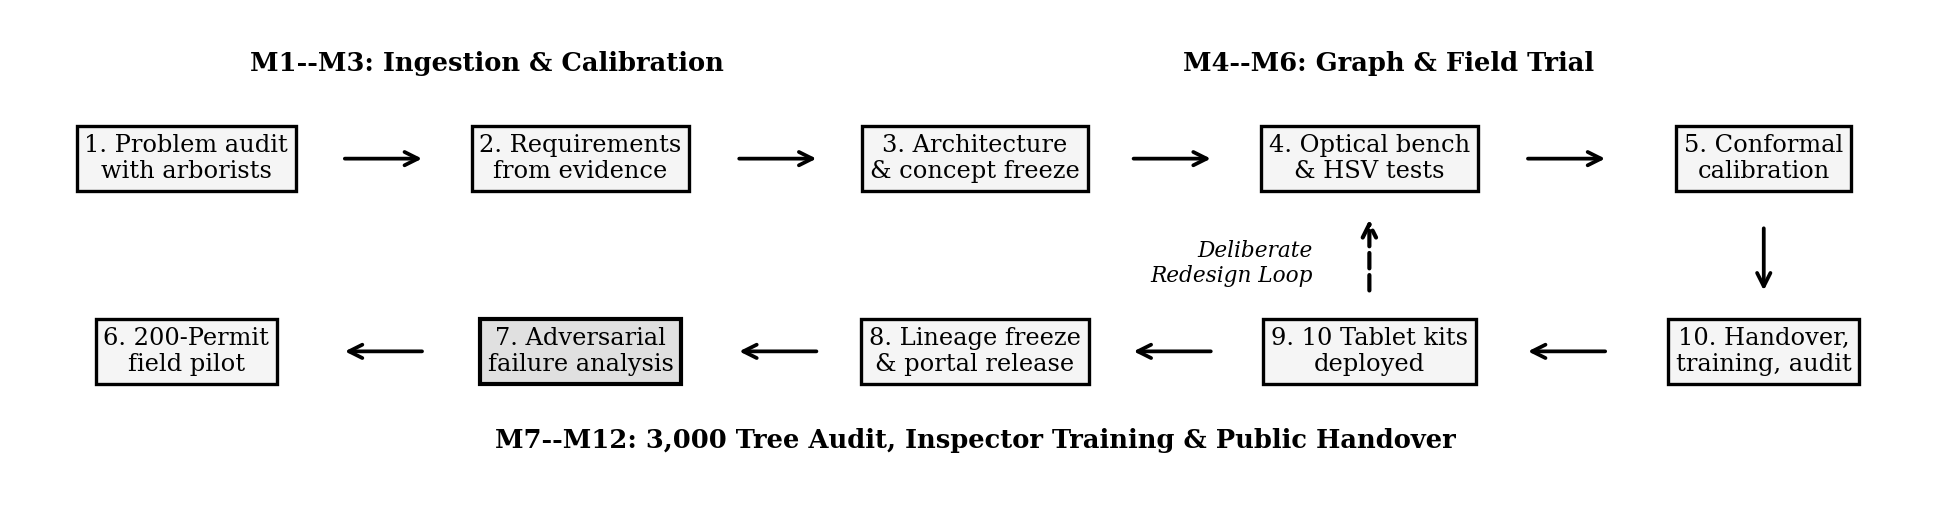
\includegraphics[width=0.96\textwidth,height=1.40in]{figures/fig8_engineering_loop.png}
  \vspace{0.2em}
  \captionof{figure}{The engineering design process as the students execute it. Stages 6 to 8 are the core of the project: the month 6 field trial is scheduled in order to produce real-world failures, and the dashed path back to optical tuning is planned iteration. A design cycle that never fails is not a design cycle.}\label{fig:loop}
\end{center}

\vspace{-0.3em}
Each stage has a named student owner and a documented output: a requirements note at stage 2, characterisation data at stage 4, a calibration certificate at stage 5, a written redesign list at stage 7, released code at stage 8, and a competency checklist at stage 10.

\vspace{0.15em}
\section{Impact and measurement}
\begin{minipage}{0.48\textwidth}
\renewcommand{\arraystretch}{0.91}
\begin{tabularx}{\textwidth}{@{}Xr@{}}
\toprule
\textsf{\textbf{\fontsize{8pt}{10pt}\selectfont Beneficiary group}} & \textsf{\textbf{\fontsize{8pt}{10pt}\selectfont Count}} \\
\midrule
Historical paper permits ingested & 3,000 \\
Validated tree records reconciled & 3,000 \\
Municipal arborists equipped with review tools & 15 \\
Urban canopy area covered & 1,450 ha \\
Compensatory saplings tracked & 9,000 \\
Direct urban population benefited & 540,000 \\
Students engaged & 4 \\
IEEE volunteers & 3 \\
Local technicians trained & 4 \\
\bottomrule
\end{tabularx}
\vspace{0.1em}
\tiny Assumptions: Coverage spans all 10 municipalities of the City of Skopje; compensatory tracking enforces statutory 3--5 saplings per felling.
\end{minipage}
\hfill
\begin{minipage}{0.48\textwidth}
\renewcommand{\arraystretch}{0.91}
\begin{tabularx}{\textwidth}{@{}Xr@{}}
\toprule
\textsf{\textbf{\fontsize{8pt}{10pt}\selectfont Metric}} & \textsf{\textbf{\fontsize{8pt}{10pt}\selectfont Target}} \\
\midrule
Cyrillic field extraction accuracy & $\ge 92.0\%$ F1 \\
Conformal coverage ($1 - \alpha$) & $\ge 95.0\%$ \\
Cadastral parcel mutation resolution & $\ge 92.0\%$ \\
Processing latency per 4-page permit & $< 4.0\text{ s}$ \\
Target auto-proposal error rate & $\le 2.0\%$ \\
Compensatory obligations tracked & $100.0\%$ \\
Staff review time per flagged case & $< 45\text{ s}$ \\
Air-gapped uptime without crash & $\ge 99.5\%$ \\
Repairs without the team & $\ge 4$ \\
\bottomrule
\end{tabularx}
\vspace{0.1em}
\tiny Measured via double-blind ground-truth validation on 200 randomly sampled permits from municipal archives.
\end{minipage}

\vspace{0.15em}
\subsection*{5.1 What this project cannot do}
\begin{itemize}[leftmargin=1.4em, itemsep=0.03em]
  \item \textbf{Treat respiratory illness.} Chronic pulmonary damage from particulate smog is irreversible. Software does not heal clinical patients.
  \item \textbf{Overturn lawful city council zoning decisions.} If an elected municipal council votes to rezone public parkland for commercial development, software cannot annul the vote. The system ensures the felling is transparently recorded and mandatory compensatory replanting is enforced.
  \item \textbf{Physically plant trees.} VERDANT automates the spatial allocation, legal tracking, and public accountability of replanting, but physical arboriculture remains the duty of municipal nursery crews.
  \item \textbf{Alter sovereign legal land boundaries.} When parcel conflicts arise between historical maps and current deeds, the system flags the dispute for the Agency for Real Estate Cadastre (AREC) rather than inventing coordinates.
  \item \textbf{Promise an immediate reduction in ambient valley pollution in twelve months.} Biological air filtration takes years as saplings mature. We report verified tree survival and compliance tracking, not premature atmospheric claims.
  \item \textbf{Change why developers clear plots.} Commercial construction pressure exists beyond software. That is beyond engineering.
\end{itemize}

\clearpage

% =============================================================
% PAGE 6: SUSTAINABILITY, RISK, STANDARDS, TEAM, PARTNER
% =============================================================
\textbf{Sustainability. Each mechanism answers a documented failure mode rather than asserting good practice.}
\vspace{0.1em}

\renewcommand{\arraystretch}{0.91}
\begin{tabularx}{\textwidth}{@{}lX@{}}
\toprule
\textsf{\textbf{\fontsize{8pt}{10pt}\selectfont Mechanism}} & \textsf{\textbf{\fontsize{8pt}{10pt}\selectfont Failure mode it addresses}} \\
\midrule
\textbf{Local municipal ownership of software} & The recurring cloud subscription cliff: when grant funds expire, cloud APIs are terminated and systems go dark \\
\textbf{Two-zone architecture with on-premise enclave} & Network security restrictions: municipal internal networks block external cloud outbound traffic \\
\textbf{Permissive open-source licensing (Apache 2.0)} & Vendor lock-in: proprietary GIS software contracts that prevent local engineers from fixing bugs \\
\textbf{Four trained local technicians} & Long-term dependence on student researchers for routine system administration and database backups \\
\textbf{Standard open-source GIS tools} & Fragile custom mobile codebases abandoned after project closeout; replaced with standard QGIS/QField tooling \\
\bottomrule
\end{tabularx}

\vspace{0.15em}
\textbf{Principal risks and mitigation.}
\vspace{0.1em}

\begin{tabularx}{\textwidth}{@{}lX@{}}
\toprule
\textsf{\textbf{\fontsize{8pt}{10pt}\selectfont Risk}} & \textsf{\textbf{\fontsize{8pt}{10pt}\selectfont Mitigation}} \\
\midrule
\textbf{Severe degradation on pre-1990 paper} & Multi-channel optical rig, CLAHE contrast equalization, and dedicated human verification fallback \\
\textbf{Cadastral parcel ID renumbering conflicts} & Recursive PostGIS DAG graph tracing parent-child parcel splits with fallback to spatial centroid intersection \\
\textbf{Citizen PII leakage during public reporting} & Automated Macedonian regex and CLASSLA NER scrubbing citizen names and national IDs (\textit{ЕМБГ}) at intake \\
\textbf{Valid-but-wrong parcel OCR errors} & Spatial context sanity checks verifying parcel street text against municipal neighborhood boundaries \\
\textbf{Municipal staff review friction} & Symmetric 1-click approve/reject interface with source page bounding box snippets \\
\bottomrule
\end{tabularx}

\vspace{0.15em}
\textbf{Standards and Regulatory Compliance.} Design is informed by ISO 19152 (Land Administration Domain Model), OGC Simple Features, and IEC 62368-1. Institutional ethics review is completed in month 1 before archival data processing. Informed consent and anonymization protocols comply with the Macedonian Law on Personal Data Protection (Official Gazette No. 42/20, transposing EU GDPR). Citizen identifiers (\textit{ЕМБГ}) are pseudonymised with keys held exclusively by the municipal archives office within the City Enclave.

\vspace{0.15em}
\section{Team}
\renewcommand{\arraystretch}{0.91}
\begin{tabularx}{\textwidth}{@{}p{3.8cm}X@{}}
\toprule
\textsf{\textbf{\fontsize{8pt}{10pt}\selectfont Member}} & \textsf{\textbf{\fontsize{8pt}{10pt}\selectfont Role and record}} \\
\midrule
\textbf{Atharve Dahima}\newline Project lead\newline ECE, MNIT Jaipur\newline IEEE Student Member & Systems architecture, containerization, CLASSLA NLP pipeline, PostGIS database architecture. Lead author on edge cyber-physical telemetry systems; experienced in Python, PyTorch, PostGIS, GDAL, and C++. \\
\textbf{Srajan Mishra}\newline Engineering co-lead\newline ECE, MNIT Jaipur\newline IEEE Student Member & Document intelligence ingestion, multi-channel optical preprocessing, Conformal Risk Control calibration suite, and React-based staff review console. \\
\textbf{Student Researchers}\newline MNIT Jaipur / Consortium & Synthetic Macedonian permit generation engine, automated test harness, bilingual documentation, impact data collection. \\
\textbf{Dr. Vishal Sharma}\newline Faculty mentor\newline Dept. of ECE, MNIT Jaipur\newline Counselor, IEEE Student Branch & Academic oversight, verification methodology, institutional financial administration, and liaison with UNDP and challenge evaluators. \\
\bottomrule
\end{tabularx}

\vspace{0.1em}
\textbf{Student learning outcomes.} Full engineering design process through field failure and redesign; distribution-free uncertainty estimation using conformal prediction; computer vision for archival document restoration; geospatial graph modeling with recursive SQL; and human-centered design for municipal workflows.

\vspace{0.15em}
\section{Community partner}
\textbf{Sector for Environmental Protection, City of Skopje} and \textbf{PE ``Parks and Greenery'' (\textit{ЈП Паркови и Зеленило})}, Bul. Ilinden 82, 1000 Skopje. Founded 1968. Responsible for public urban forestry, municipal nurseries, and green cadastre maintenance across the 10 municipalities of the City of Skopje. (Formal letter of support requested through UNDP challenge matchmaking).

\clearpage

% =============================================================
% PAGE 7: PARTNER ROLE, STAGED BUDGET (PROTOTYPE $10K + PILOT $30K)
% =============================================================
\renewcommand{\arraystretch}{0.91}
\begin{tabularx}{\textwidth}{@{}lXlX@{}}
\toprule
\textsf{\textbf{\fontsize{8pt}{10pt}\selectfont Stage}} & \textsf{\textbf{\fontsize{8pt}{10pt}\selectfont Municipal Partner Role}} & \textsf{\textbf{\fontsize{8pt}{10pt}\selectfont Fallback if Delayed}} & \textsf{\textbf{\fontsize{8pt}{10pt}\selectfont Expected Date}} \\
\midrule
\textbf{Co-Design} & Nominates priority permit folders, shares permit schema & Use synthetic permit generator and open legal templates & Month 1 \\
\textbf{Data Access} & Provides sample anonymized scans / digital PDFs and Cadastre export & Calibrate on synthetic Cyrillic corpus + open WFS data & Month 2 \\
\textbf{Review Testing} & Designates staff arborists to test 1-click diff review console & Run remote synthetic review sessions with UKIM liaison & Month 5 \\
\textbf{Pilot Integration} & Hosts on-premise City Enclave node in municipal records depot & Maintain hosted sandbox container for remote verification & Month 6--8 \\
\bottomrule
\end{tabularx}

\vspace{0.15em}
Municipal inspection teams face severe administrative backlogs. VERDANT is designed to add capacity rather than consume it: the software runs locally without cloud subscription fees, presents proposals as clear side-by-side diffs, and integrates with standard open-source GIS tools. Co-design ensures municipal staff retain veto power over every proposed database mutation.

\vspace{0.15em}
\section{Budget: Staged Prototype (\$10,000) and Pilot Blueprint (\$30,000)}
The funding is strictly decoupled into two phases: the **Prototype Phase (\$10,000 USD)**, focused exclusively on software engineering, model calibration, synthetic data, and benchmark validation; and the **Pilot Extension Blueprint (\$30,000 USD)**, staged for on-site municipal deployment through 31 December 2027.

\vspace{0.1em}
\subsection*{7.1 Prototype Phase Budget: Exactly USD 10,000}
\renewcommand{\arraystretch}{0.91}
\begin{tabularx}{\textwidth}{@{}llXr@{}}
\toprule
\textsf{\textbf{\fontsize{8pt}{10pt}\selectfont Line}} & \textsf{\textbf{\fontsize{8pt}{10pt}\selectfont Category}} & \textsf{\textbf{\fontsize{8pt}{10pt}\selectfont Technical Purpose and Justification}} & \textsf{\textbf{\fontsize{8pt}{10pt}\selectfont USD}} \\
\midrule
1 & Compute \& GPU Testbeds & GPU cloud compute instances for local model fine-tuning and OCR benchmarking & 3,200 \\
2 & Annotation \& Linguistics & Double-annotation of 200 real Macedonian permit samples by language specialists & 2,800 \\
3 & Enclave Security \& Sandbox & On-premise Docker container staging, PII masking validation, penetration testing & 2,200 \\
4 & Documentation \& Packaging & Bilingual Macedonian/Albanian user manuals, open-source packaging, CI/CD automation & 1,800 \\
\midrule
\textbf{Total} & \textbf{Prototype Phase} & \textbf{Direct Prototype Implementation Budget (100\% Permissive Open-Source)} & \textbf{10,000} \\
\bottomrule
\end{tabularx}

\vspace{0.2em}
\subsection*{7.2 Itemized prototype expense justification}
\begin{itemize}[leftmargin=1.4em, itemsep=0.03em]
  \item \textbf{Line 1: Compute \& GPU Testbeds (\$3,200):} Dedicated GPU compute time (NVIDIA A10G/RTX 4090 instances) for fine-tuning PaddleOCR and Tesseract 5 on historical Cyrillic typefaces, training the synthetic permit generator, and running the Learn-then-Test conformal calibration suite across 10,000 simulated permit permutations.
  \item \textbf{Line 2: Annotation \& Linguistic Verification (\$2,800):} Honoraria for Macedonian-speaking domain reviewers and linguists to perform double-blind ground-truth annotation across 200 real archival permits, verifying botanical species aliases, handwritten parcel notations, and official seal boundaries.
  \item \textbf{Line 3: Enclave Security \& Sandbox Testing (\$2,200):} Dedicated local hardware testbed simulating the municipal enclave environment, verifying 100\% offline execution, PII masking accuracy under North Macedonia's Law on Personal Data Protection, and audit log tamper-resistance.
  \item \textbf{Line 4: Documentation, Translation \& Packaging (\$1,800):} Translation of municipal IT runbooks and arborist user guides into Macedonian and Albanian; open-source release packaging under Apache-2.0; automated container builds and testing pipelines.
\end{itemize}

\clearpage

% =============================================================
% PAGE 8: PILOT BLUEPRINT ($30K), CHECKLIST, RISK, REFERENCES
% =============================================================
\subsection*{7.3 Pilot Deployment Blueprint: USD 30,000 Staged Follow-on (Through Dec 2027)}
If selected by UNDP and the City of Skopje for the subsequent pilot stage, funding is allocated strictly across four milestone-gated operational packages:

\vspace{0.1em}
\renewcommand{\arraystretch}{0.89}
\begin{tabularx}{\textwidth}{@{}llXr@{}}
\toprule
\textsf{\textbf{\fontsize{8pt}{10pt}\selectfont Milestone}} & \textsf{\textbf{\fontsize{8pt}{10pt}\selectfont Operational Package}} & \textsf{\textbf{\fontsize{8pt}{10pt}\selectfont Implementation Scope and Deliverable}} & \textsf{\textbf{\fontsize{8pt}{10pt}\selectfont USD}} \\
\midrule
M1 (M7--M9) & On-Site Municipal Staging & Deploying intake workstation in City records depot; AREC adapter integration & 8,500 \\
M2 (M10--M12) & Staff Training \& Usability & Conducting arborist verification workshops, bilingual manuals, competency audit & 6,500 \\
M3 (M13--M18) & QField Mobile Workflows & Deploying open-source QField mobile profiles on existing municipal tablets & 5,000 \\
M4 (M19--M24) & Long-Term Maintenance & Model re-calibration, database indexing, software support through Dec 2027 & 10,000 \\
\midrule
\textbf{Total} & \textbf{Pilot Extension} & \textbf{Complete 18-Month Municipal Pilot Follow-On Funding Allocation} & \textbf{30,000} \\
\bottomrule
\end{tabularx}

\vspace{0.2em}
\subsection*{8. Preparation for the November 19 Q\&A Session}
The team has registered for the November 19 live technical session to resolve four critical operational dependencies:
\begin{enumerate}[leftmargin=1.4em, itemsep=0.02em]
  \item \textbf{Permit Format:} Clarify whether the City already holds digital PDF scans from prior scanning projects, which would eliminate scanner hardware needs entirely.
  \item \textbf{Cadastre Interface:} Determine whether the *Zelen Katastar* is accessible via PostGIS database dumps, GeoPackage exports, or live WFS/REST endpoints.
  \item \textbf{Sample Benchmark Data:} Request access to an anonymized sample of historical permits to calibrate the Phase 1 Zindi evaluation baseline.
  \item \textbf{November 30 Dataset Window:} Confirm protocols for contributing the open-source synthetic Cyrillic permit dataset to the competition ecosystem.
\end{enumerate}

\vspace{0.2em}
\subsection*{8.1 Pre-registered pilot success criteria}
\begin{itemize}[leftmargin=1.4em, itemsep=0.02em]
  \item \textbf{Backlog Ingestion:} Ingest and extract all 3,000 historical permits within 30 days of municipal deployment.
  \item \textbf{Review Time Reduction:} Reduce per-permit verification time from manual 45 minutes to under 2 minutes.
  \item \textbf{Proposal Quality:} Achieve $\ge 85\%$ staff acceptance rate on automated cadastral update proposals.
  \item \textbf{Zero Unreviewed Mutations:} 100\% of Cadastre database commits verified by authorized municipal staff.
\end{itemize}

\vspace{0.2em}
\textsf{\textbf{\fontsize{7.5pt}{9pt}\selectfont References.}}
\fontsize{7.5pt}{9pt}\selectfont
[1] City of Skopje \& PE ``Parks and Greenery'', \textit{Zelen Katastar na Grad Skopje}, Official Municipal Registry, 2020--2024.
[2] V. Vovk, A. Gammerman, and G. Shafer, \textit{Algorithmic Learning in a Random World}, Springer, 2005.
[3] A. N. Angelopoulos and S. Bates, ``A gentle introduction to conformal prediction,'' \textit{arXiv:2107.07511}, 2021.
[4] CLARIN.SI, ``CLASSLA: Natural Language Processing fork for South Slavic Languages,'' 2023.
[5] Republic of North Macedonia, \textit{Law on Personal Data Protection}, Official Gazette No. 42/20, 2020.
[6] UNDP North Macedonia, \textit{Skopje Urban Green Cadastre Technical Baseline Assessment}, 2021.

\end{document}
